\documentclass[10pt, a4paper]{article}
\usepackage[utf8]{inputenc}
\usepackage[T1]{fontenc}
\usepackage[spanish]{babel} % Para separación de sílabas en español
\usepackage{geometry}
\geometry{a4paper, margin=2cm} % Márgenes cómodos

% Paquetes CRUCIALES para tu trabajo
\usepackage{graphicx} % Para incluir imágenes si las hay
\usepackage{hyperref} % Para hypervínculos en el índice y referencias
\hypersetup{
    colorlinks=true,
    linkcolor=blue,
    filecolor=magenta,
    urlcolor=cyan,
    pdftitle={TP Legislación - IA},
}
\usepackage{csquotes} % Para comillas correctas según el idioma
\usepackage[style=apa, backend=biber, language=auto]{biblatex} % Bibliografía APA
\usepackage{tabularx} % Para tablas con ancho de columna ajustable
\usepackage{booktabs} % Para líneas de tabla más profesionales
\usepackage{titling} % Para personalizar la portada

\DeclareLanguageMapping{spanish}{spanish-apa} % Mapea el idioma 'spanish' a la variante de estilo 'spanish-apa'
\addbibresource{bibliografica.bib} % Apunta a tu archivo .bib

% Metadatos del documento
\title{Inteligencia Artificial en Argentina: Un Análisis Jurídico desde la Constitución Nacional y el Código Civil y Comercial}
\author{
    Mayra Garcia \\
    Facundo Longin \\
    Elías Aires  \\
    Juan Cruz Yorio \\
    Matias Pormi
}
\date{} % <-- Esto elimina la fecha de la portada

% --- Personalización de la portada con 'titling' ---
\pretitle{\begin{center}\LARGE\bfseries}
\posttitle{\par\end{center}\vspace{1.5cm}}
\preauthor{\begin{center}\large\bfseries Integrantes Grupo 5 \par\vspace{0.5cm}\normalfont}
\postauthor{\end{center}}

\begin{document}

\maketitle % Genera la portada

\vfill % Empuja la imagen hacia abajo, ocupando el espacio disponible

\noindent\makebox[\textwidth]{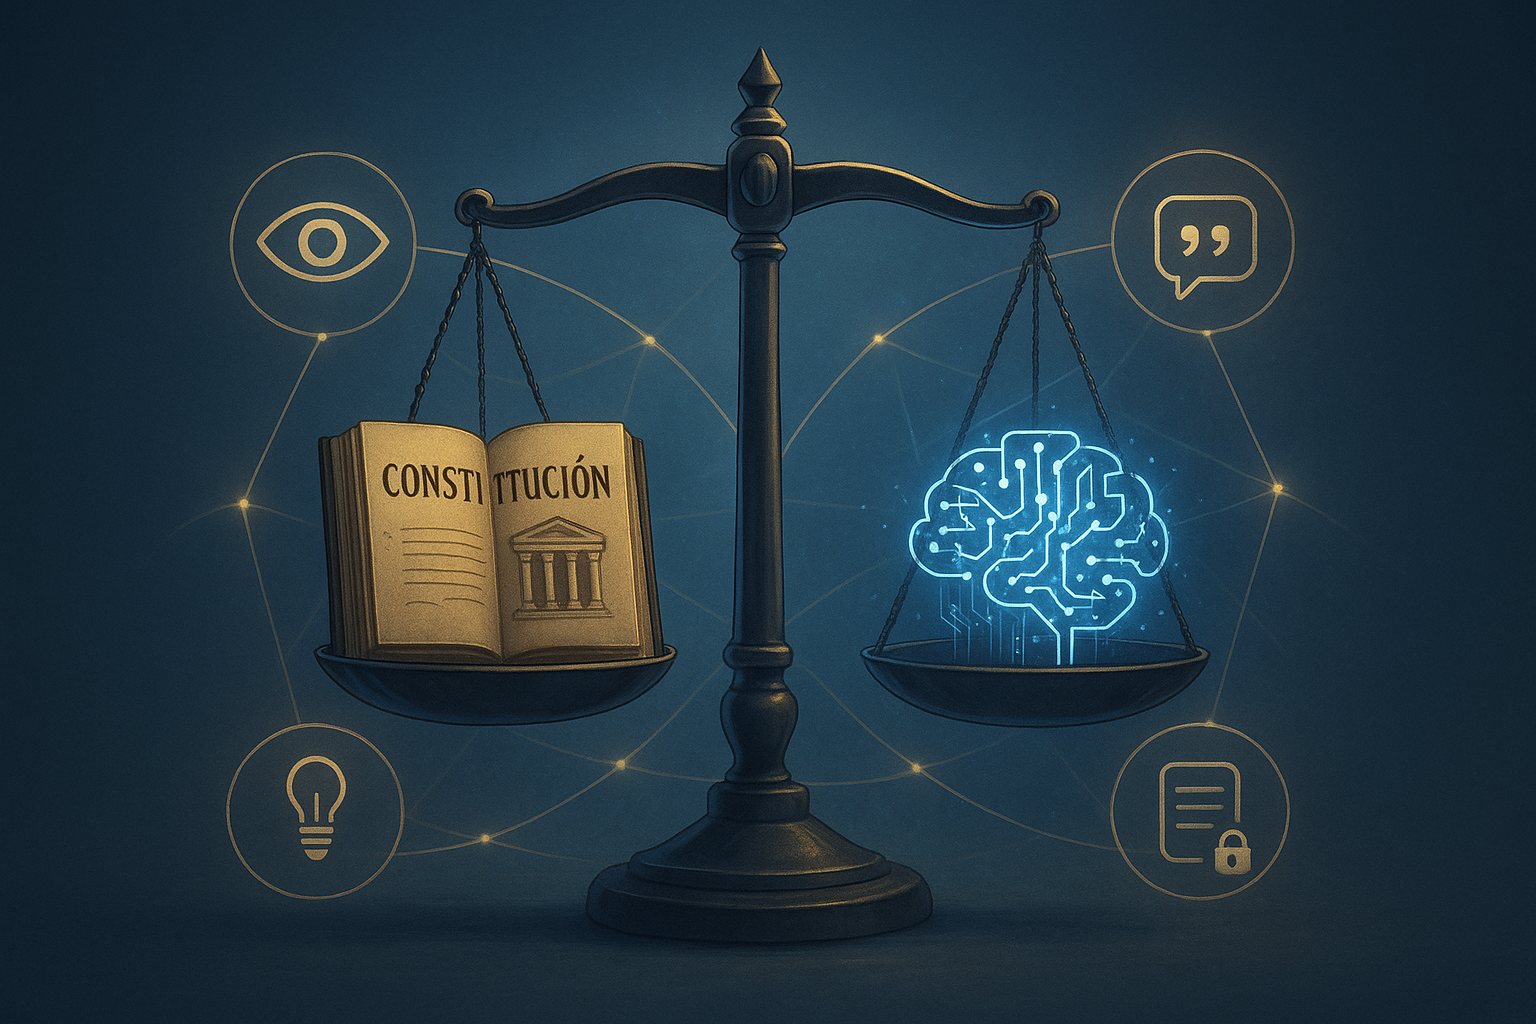
\includegraphics[width=\textwidth]{./imagen_portada.png}}


\newpage % Fuerza un salto de página después del índice
\tableofcontents % Genera el índice automáticamente
\newpage % Fuerza un salto de página después del índice
\twocolumn % <-- A partir de aquí, todo será en dos columnas

\label{sec:Resumen}
\begin{abstract}
Este trabajo práctico analiza los desafíos que la Inteligencia Artificial (IA) plantea al marco jurídico argentino, tomando como caso de estudio el artículo \enquote{La Arquitectura Constitucional de la Innovación con IA: Red de Protección para el Desarrollo Tecnológico Responsable}. El objetivo principal es examinar cómo los principios fundamentales del derecho privado y constitucional contenidos en las primeras siete unidades de la obra \enquote{Legislación - Lecciones de Derecho} pueden aplicarse para regular esta tecnología disruptiva. La metodología consiste en un análisis jurídico-doctrinario que relaciona de manera crítica cada capítulo del libro (desde el concepto de Derecho hasta los Derechos Reales) con los problemas específicos que surgen de la IA, como la responsabilidad por daños de sistemas autónomos, la validez de los actos jurídicos celebrados por agentes artificiales y la protección de los datos personales. Desde un \emph{enfoque ingenieril}, se concluye que el desarrollo técnico de la IA en Argentina debe incorporar por defecto principios de \emph{privacy by design} y \emph{transparencia algorítmica} para alinearse con las garantías constitucionales y evitar incurrir en responsabilidad civil o contractual. El hallazgo central del trabajo es que la Constitución Nacional de 1853, a través de una \emph{interpretación evolutiva} de sus cláusulas (arts. 19, 14, 42 y 33), provee una red de protección suficientemente robusta y flexible para fomentar la innovación tecnológica responsable, sin necesidad de una reforma legal inmediata, sirviendo como guía para una eventual ley específica de IA.

\vspace{0.5cm}
\noindent \textbf{Palabras clave:} Inteligencia Artificial, Derecho Argentino, Interpretación Evolutiva, Constitución Nacional, Responsabilidad Algorithmica, Ética en la Ingeniería.
\end{abstract}

\section{Introducción}
\label{sec:introduccion}

La inteligencia artificial (IA) ha irrumpido en el siglo XXI no solo como una herramienta tecnológica, sino como una fuerza disruptiva que redefine industrias, interacciones sociales y, de manera crucial, los marcos normativos que rigen las sociedades contemporáneas. Su desarrollo vertiginoso presenta desafíos jurídicos complejos que tensionan los conceptos tradicionales del derecho, tales como la personalidad jurídica, la responsabilidad civil, la privacidad y la validez de los actos voluntarios. Argentina, en su aspiración de convertirse en un hub tecnológico global, no es ajena a este debate, que se manifiesta en una creciente producción legislativa y doctrinaria orientada a encontrar un equilibrio entre la innovación desregulada y la protección irrestricta de los derechos fundamentales.

El presente trabajo se enmarca en el análisis de este fenómeno a partir del artículo periodístico de \textcite{articulo_ia}, titulado \enquote{La Arquitectura Constitucional de la Innovación con IA: Red de Protección para el Desarrollo Tecnológico Responsable}. Este artículo, de origen argentino y reciente publicación, resulta particularmente oportuno para el análisis, ya que propone una solución inherentemente jurídica: la aplicación de una \emph{interpretación evolutiva} de la Constitución Nacional de 1853 para dar respuesta a los problemas inéditos que plantea la IA, sin necesidad de acudir inicialmente a una reforma legal integral.

El objetivo central de esta investigación es realizar un análisis crítico y detallado que permita \emph{relacionar} los postulados del artículo mencionado con los contenidos de las primeras siete unidades del libro de texto, \enquote{Legislación - Lecciones de Derecho}. Se procederá a un examen secuencial de cada capítulo (El Derecho, El Sistema Jurídico, La Constitución, Persona, Hechos y Actos Jurídicos, Obligaciones y Derechos Reales), explorando cómo los principios allí establecidos interactúan y se adaptan a los desafíos específicos de la IA.

Adicionalmente, y en cumplimiento de la consigna práctica, se incorporará un \emph{enfoque ingenieril} desde la perspectiva de la ingeniería en sistemas. Este enfoque complementará el análisis jurídico, examinando las implicancias prácticas que estos principios legales tienen en el ciclo de vida del desarrollo de software, la gestión de proyectos de IA y la implementación de mecanismos de ética por diseño (\emph{ethics by design}).

\section{Desarrollo del Marco Teórico}
\label{sec:desarrollo}

\subsection{Capítulo I: ``El Derecho''}
\label{subsec:derecho}

El Capítulo I de la obra \textcite{libro_legislacion} establece que el Derecho es un sistema dinámico de normas que regulan la convivencia social, con el fin de alcanzar valores fundamentales como la \emph{justicia, el orden, la seguridad y la paz}. Estas normas jurídicas, coercibles y coactivas, se diferencian de otras (morales, religiosas, sociales) por su carácter imperativo y por ser creadas y garantizadas por el Estado para organizar la vida en sociedad de manera pacífica y justa.

La irrupción de tecnologías disruptivas como la Inteligencia Artificial (IA) representa un desafío sin precedentes para estos conceptos fundacionales. El artículo ``La Arquitectura Constitucional de la Innovación con IA'' plantea que la tensión entre innovación tecnológica y regulación puede resolverse mediante una \textbf{interpretación evolutiva} de la Constitución Nacional, la cual provee una \emph{red de protección} basada en seis nodos constitucionales clave. Esta red permite que el marco normativo existente se adapte para abordar realidades donde actores no humanos (sistemas de IA) toman decisiones autónomas, sin necesidad de abandonar los principios esenciales del Derecho identificados en el Capítulo I.

\subsubsection*{Los Seis Nodos Constitucionales y su Relación con el Concepto de Derecho:}
El artículo periodístico propone que la CN de 1853, a través de una interpretación dinámica, ofrece un marco completo para regular la IA. Esta \emph{arquitectura constitucional} se sustenta en los siguientes nodos, cada uno de los cuales interactúa con los valores y funciones del Derecho:

\begin{enumerate}
    \item \textbf{Art. 19 CN (Acciones privadas):} Protege las ``acciones privadas que de ningún modo ofendan al orden y a la moral pública, ni perjudiquen a un tercero''. En la era digital, este artículo se reinterpreta para amparar la privacidad y autonomía de las personas frente a intromisiones de sistemas de IA, reflejando el valor jurídico del \textbf{orden} y la \textbf{seguridad} personal. El Derecho, como ordenador de la convivencia, debe garantizar que el desarrollo tecnológico no vulnere este espacio de libertad individual.

    \item \textbf{Art. 14 CN (Derecho a ejercer industria lícita):} Ampara la innovación y el desarrollo tecnológico, incluida la IA. Este nodo representa el valor \textbf{poder} (capacidad de innovar y crear) dentro del esquema de valores jurídicos. Sin embargo, el artículo destaca que este derecho no es absoluto y encuentra su límite en el mismo Art. 19 (no dañar a terceros) y en el \textbf{orden público}. El Derecho debe así balancear dos de sus valores fundacionales: fomentar el progreso (\textbf{poder}) y proteger la convivencia (\textbf{seguridad} y \textbf{paz}).

    \item \textbf{Art. 42 CN (Derechos de usuarios y consumidores):} Establece la obligación de las autoridades de proveer protección contra distorsiones del mercado y de controlar los monopolios. aplicado a la IA, este nodo exige \textbf{transparencia algorítmica}, rendición de cuentas y protección contra prácticas abusivas o discriminatorias por parte de quienes desarrollan o despliegan estas tecnologías. Refleja el valor de la \textbf{justicia} en las relaciones de consumo y el rol del Estado como garante de equidad.

    \item \textbf{Protección de Datos Personales (Derivado del Art. 33 CN - Derechos Implícitos):} Aunque no explícito en el texto, se reconoce como un derecho fundamental derivado de los Arts. 19 y 33 CN. Este nodo es crucial para la IA, cuyo combustible son los datos. Exige principios de \textbf{minimización, finalidad y consentimiento informado} en el tratamiento de datos para entrenar sistemas de IA, vinculándose directamente con el valor de la \textbf{seguridad} jurídica de las personas.

    \item \textbf{Art. 28 CN (Principio de Razonabilidad):} Establece que los principios, garantías y derechos reconocidos por la CN no podrán ser alterados por las leyes que reglamenten su ejercicio. Toda regulación o limitación estatal a la IA debe superar el test de razonabilidad: finalidad legítima, idoneidad, necesidad y proporcionalidad. Este nodo es la herramienta jurídica primordial para asegurar que cualquier normativa sobre IA sea \textbf{justa} y no arbitraria, protegiendo así la certeza del derecho.

    \item \textbf{Art. 33 CN (Derechos Implícitos):} Funciona como una cláusula abierta que permite reconocer nuevos derechos no enumerados expresamente. El artículo periodístico argumenta que aquí pueden fundarse derechos emergentes como el ``derecho a la identidad digital'', el ``derecho a la no discriminación algorítmica'' o el ``derecho al desarrollo tecnológico''. Este nodo es la máxima expresión del Derecho como sistema \textbf{vivo} y en evolución, capaz de adaptarse a realidades futuras imprevistas por el constituyente, siempre en busca de la \textbf{justicia}.
\end{enumerate}

\subsubsection*{Conclusión parcial:}
El análisis del artículo periodístico a la luz de los conceptos del Capítulo I demuestra que la \emph{red de protección constitucional} basada en los seis nodos no es una creación novedosa, sino la aplicación coherente de la naturaleza misma del Derecho: un sistema dinámico orientado por valores. La \textbf{interpretación evolutiva} permite que estos principios constitucionales interactúen para regular la IA, balanceando la innovación con la protección de derechos, el \textbf{poder} con la \textbf{seguridad}, y la libertad individual con el \textbf{orden} público. Así, el Derecho demuestra su capacidad de mantener su esencia mientras regula realidades tecnológicas completamente nuevas.

\subsection{Capítulo II: ``El Sistema Jurídico''}
\label{subsec:sistema}

El sistema jurídico argentino se estructura bajo el principio de \textbf{supremacía constitucional} (Art. 31 CN), donde la CN \parencite{constitucion} es la norma fundamental que integra y da coherencia a todo el ordenamiento. El artículo periodístico analizado destaca que, ante la ausencia de una ley específica de IA, la regulación debe articularse mediante una \textbf{interpretación sistemática} que combine diversas fuentes normativas bajo el paraguas constitucional.

La pirámide de Kelsen ofrece el marco para entender cómo se regula la IA:
\begin{itemize}
    \item \textbf{CN y Tratados Internacionales:} Establecen derechos fundamentales (privacidad, no discriminación) que limitan el desarrollo y uso de IA.
    \item \textbf{Leyes Nacionales:} Normas como la Ley 25.326 (Protección de Datos) y el CCyC contienen principios aplicables por analogía.
    \item \textbf{Reglamentos:} El Poder Ejecutivo puede emitir disposiciones específicas dentro de su competencia.
\end{itemize}

\subsubsection*{Ejemplo:}
Un algoritmo de contratación discrimina por género. El sistema jurídico responde:
1) Aplicando la CN (Art. 16) y tratados contra la discriminación.
2) Utilizando la Ley 23.592 para sancionar.
3) Interpretando evolutivamente estos marcos para cubrir el vacío legal, creando jurisprudencia.

\subsubsection*{Conclusión:}
El sistema jurídico vigente, con la CN como eje, permite una regulación preliminar de la IA mediante interpretación coherente de normas existentes. Sin embargo, la falta de una ley específica genera inseguridad, destacando la necesidad de una regulación ad hoc que ordene el tema sistemáticamente.
\subsection{Capítulo III: ``La Constitución de la Nación Argentina''}
\label{subsec:constitucion}

Este capítulo se centra en los mecanismos constitucionales específicos que complementan el marco analizado anteriormente, proporcionando herramientas concretas para la regulación de la inteligencia artificial.

\subsubsection*{Ejemplo práctico - Articulación de garantías constitucionales:}
Una plataforma de delivery que utiliza IA para gestionar repartos establece diferencias salariales entre repartidores de diferentes barrios mediante un algoritmo opaco. Los trabajadores afectados podrían accionar mediante:
\begin{itemize}
    \item \textbf{Amparo colectivo} (Art. 43 CN) por afectación de derechos laborales
    \item \textbf{Habeas data} (Art. 43 CN) para acceder a los criterios algorítmicos
    \item Protección de \textbf{derechos de incidencia colectiva} (Art. 14 CCyC)
\end{itemize}

Este caso demuestra cómo los diferentes instrumentos constitucionales interactúan para proteger derechos vulnerados por sistemas de IA, incluso sin legislación específica.

\subsubsection*{Conclusión:}
La CN provee una red de protección integral a través de la articulación de sus diferentes instrumentos procesales y sustantivos, permitiendo abordar casos complejos de IA mediante la aplicación conjunta de diversas garantías constitucionales.
\subsection{Capítulo IV: ``Persona''}
\label{subsec:persona}

El concepto de persona en el Código Civil y Comercial de la Nación \parencite{ccyc} constituye uno de los pilares fundamentales del sistema jurídico argentino, regulado en los arts. 22 a 25. Según estas disposiciones, solo las personas humanas y jurídicas son consideradas sujetos de derecho, gozando de capacidad para adquirir derechos y contraer obligaciones. Sin embargo, este marco normativo evidencia importantes limitaciones ante los avances tecnológicos, particularmente en el ámbito de la inteligencia artificial (IA), donde sistemas autónomos pueden realizar acciones con consecuencias jurídicas sin encuadrar en las categorías tradicionales de persona.

\subsubsection*{Limitaciones del CCyC frente a la IA:}
\begin{itemize}
    \item \textbf{Art. 22 CCyC:} Establece que "Son personas todos los entes susceptibles de adquirir derechos o contraer obligaciones". Esta definición excluye expresamente a los sistemas de IA, al requerir un sustrato biológico (persona humana) o una construcción jurídica (persona jurídica).
    \item \textbf{Art. 23 CCyC:} Define el inicio de la existencia de la persona humana, requisitos que obviamente no pueden ser satisfechos por entidades artificiales.
    \item \textbf{Vacío legal:} La imposibilidad de atribuir personalidad jurídica a sistemas autónomos genera un déficit de responsabilidad cuando estos causan daños sin intervención humana directa.
\end{itemize}

\subsubsection*{Ejemplo práctico - Sistema de IA en gestión financiera:}
Un algoritmo de inversión autónomo gestiona carteras de valores en el mercado bursátil argentino. Tras una falla en su diseño, realiza operaciones masivas que provocan pérdidas significativas a inversionistas y afectan la estabilidad del mercado. El análisis bajo el CCyC revela:

\begin{itemize}
    \item \textbf{Falta de sujeto responsable:} El algoritmo no es persona según el Art. 22 CCyC, por lo que no puede ser considerado responsable civilmente.
    \item \textbf{Distribución de responsabilidad:} Los afectados deberán demandar a los desarrolladores, propietarios o usuarios del sistema bajo figuras indirectas.
    \item \textbf{Art. 1757 CCyC:} Podría aplicarse por analogía, considerando al sistema de IA como "cosa riesgosa", haciendo responsable a su "guardián".
    \item \textbf{Responsabilidad solidaria:} Ante la dificultad de determinar la proporción exacta de responsabilidad, podría aplicarse el principio de responsabilidad solidaria entre fabricante, programador y propietario.
\end{itemize}

\subsection{Capítulo V: ``Hechos y Actos Jurídicos''}
\label{subsec:hechos_actos}

El Código Civil y Comercial de la Nación (CCyCN) regula en su Título IV los hechos y actos jurídicos, estableciendo las bases para entender cómo se generan, modifican y extinguen las relaciones jurídicas. Según el Art. 257 CCyCN, el \textbf{hecho jurídico} es el acontecimiento que, conforme al ordenamiento jurídico, produce el nacimiento, modificación o extinción de relaciones o situaciones jurídicas. Estos pueden ser naturales (ej. un desastre natural) o humanos (ej. un contrato). Por su parte, el \textbf{acto jurídico} (Art. 259 CCyCN) es un acto voluntario lícito que tiene por fin inmediato la adquisición, modificación o extinción de relaciones o situaciones jurídicas. La voluntad, esencial en los actos jurídicos, debe manifestarse con discernimiento, intención y libertad (Art. 260 CCyCN).

Sin embargo, la irrupción de la inteligencia artificial (IA) desafía estas categorías tradicionales. Los sistemas de IA, al operar con autonomía, realizan acciones que pueden generar efectos jurídicos sin encuadrar perfectamente en las figuras de hecho o acto jurídico, ya que carecen de voluntad humana pero pueden simularla. El artículo periodístico analizado propone que esta tensión debe resolverse mediante una \textbf{interpretación evolutiva} de las normas existentes, extendiendo los conceptos tradicionales para abarcar los nuevos desafíos tecnológicos sin necesidad de reformas legislativas inmediatas.

\subsubsection*{Ejemplo práctico - Contrato celebrado por IA:}
Un sistema de IA utilizado por una empresa de comercio electrónico celebra contratos de compraventa de forma autónoma, ajustando precios y condiciones en tiempo real. Tras una falla algorítmica, ofrece productos con precios erróneamente bajos, causando pérdidas económicas a la empresa. El análisis bajo el CCyCN revela:
\begin{itemize}
    \item \textbf{Falta de voluntad válida:} La IA carece de discernimiento e intención (Art. 260 CCyCN), por lo que el acto no encaja perfectamente como acto jurídico.
    \item \textbf{Imposibilidad de aplicar vicios:} No es posible alegar error (Art. 265 CCyCN) o dolo (Art. 272 CCyCN) contra la IA, ya que estos requieren una voluntad humana viciada.
    \item \textbf{Responsabilidad indirecta:} La empresa podría ser responsable como "guardiana" de la IA bajo el Art. 1757 CCyCN (cosa riesgosa), pero este artículo no está diseñado para actos jurídicos autónomos.
\end{itemize}
\subsection{Capítulo VI: ``Obligaciones''}
\label{subsec:obligaciones}

El CCyC regula en los arts. 724 a 927 el régimen de obligaciones, distinguiendo entre fuentes contractuales y extracontractuales. Los sistemas de IA plantean desafíos particulares en la imputación de responsabilidad, especialmente en casos donde la autonomía algorítmica dificulta establecer nexo causal y culpa, tal como analiza el artículo periodístico.

\subsubsection*{Ejemplo práctico - Responsabilidad por algoritmo crediticio:}
Un sistema de scoring crediticio basado en IA deniega automáticamente solicitudes de crédito a personas de determinado perfil socioeconómico. El análisis legal revela:

\begin{itemize}
    \item \textbf{Art. 1710 CCyC:} Responsabilidad por daños causados por el riesgo o vicio de las cosas
    \item \textbf{Art. 1768 CCyC:} Carga de la prueba inversa en casos de afectación de derechos de incidencia colectiva
    \item \textbf{Art. 1774 CCyC:} Responsabilidad solidaria entre desarrolladores, implementadores y usuarios del sistema
\end{itemize}

\subsubsection*{Vinculación con el artículo periodístico:}
El artículo sostiene que el principio de razonabilidad (Art. 28 CN) obliga a distribuir la carga probatoria de manera equilibrada, favoreciendo a los afectados por decisiones algorítmicas opacas. La interpretación evolutiva del art. 42 CN sobre derechos del consumidor podría exigir la transparencia algorítmica como obligación esencial.

\subsection{Capítulo VII: ``Derechos Reales''}
\label{subsec:derechos_reales}

El CCyC regula en los arts. 1886 a 1972 los derechos reales, que otorgan a su titular un poder jurídico, de estructura legal, que se ejerce directamente sobre su objeto en forma autónoma y que atribuye a su titular las facultades de persecución y preferencia, y las demás provistas en este código, derechos los cuales son oponibles \textit{erga omnes}. Estos abarcan, entre otros, la propiedad, el usufructo, la servidumbre, la hipoteca y la prenda.  

Ahora bien, los desafíos que plantea la inteligencia artificial en torno a la propiedad de datos y a las creaciones generadas por algoritmos \textbf{no constituyen derechos reales en sentido técnico}. La \textit{propiedad intelectual} cuenta con un régimen específico (Ley 11.723 y art. 17 CN), y los \textit{datos personales} son protegidos como derechos personalísimos mediante la Ley 25.326 y el art. 43 CN (habeas data).  

No obstante, puede establecerse una \textbf{analogía}: tanto los derechos reales como estos regímenes especiales comparten la tensión entre el \textit{dominio individual} (el ejercicio exclusivo que tiene el titular sobre un bien u objeto) y la \textit{función social} (los límites que impone el ordenamiento para proteger el interés general). En la era digital, esta tensión se expresa en el control sobre obras creadas por IA, en la titularidad de bases de datos y en el uso de información personal para entrenar sistemas algorítmicos.  

\subsubsection*{Ejemplo práctico - Propiedad en el Metaverso}
En los entornos virtuales (metaverso), los usuarios adquieren terrenos, activos o bienes digitales que, aunque no encuadran como derechos reales clásicos, se consideran bienes incorporales con valor económico. La IA interviene tanto en la \textbf{creación} de estos objetos digitales (diseños, entornos, experiencias) como en su \textbf{gestión} mediante algoritmos y contratos inteligentes.  

\subsubsection*{Vinculación con el artículo periodístico}
En línea con lo planteado por Lerer, la Constitución Nacional, a través de los arts. 14 (ejercer industria lícita), 42 (derechos de consumidores y usuarios) y 33 (reconocimiento de derechos implícitos), ofrece un marco de protección para estos \textbf{derechos emergentes}, equilibrando innovación tecnológica con la defensa de la persona y el interés público.


\onecolumn % <-- Volvemos a una columna y se inserta un salto de página

\section{Enfoque Ingenieril}
\label{sec:enfoque_ingenieril}

Desde la perspectiva de la ingeniería en sistemas, el desarrollo de inteligencia artificial debe incorporar principios de diseño ético y cumplimiento legal desde sus etapas iniciales. El artículo periodístico analizado proporciona un marco conceptual que puede traducirse en prácticas ingenieriles concretas.

\subsection{Implementación Técnica de Garantías Constitucionales}
Las garantías analizadas requieren traducción a requisitos técnicos:

\begin{table*}[h]
\centering
\caption{Traducción de garantías constitucionales a implementación técnica}
\begin{tabularx}{\textwidth}{lX}
\toprule
\textbf{Garantía Constitucional} & \textbf{Implementación Técnica} \\
\midrule
Art. 19 CN (Privacidad) & Cifrado de extremo a extremo (end-to-end encryption), técnicas de anonimización y pseudoanonimización de datos. \\
\addlinespace
Art. 42 CN (Transparencia) & Creación de \textit{Model Cards} y \textit{Dataset Sheets} para documentar modelos y datos, uso de control de versiones para trazabilidad. \\
\addlinespace
Art. 43 CN (Amparo) & Implementación de un sistema de registro de eventos (logging) exhaustivo y sistemas de reversión (rollback) automáticos ante fallos críticos. \\
\bottomrule
\end{tabularx}
\end{table*}

\section{Conclusión}
\label{sec:conslusion}

El articulo mencionado, junto con los temas de \enquote{Legislación - Lecciones de Derecho} trae a la luz el hecho de que no hace falta que exista un marco legal moderno para que un sector nuevo, como lo es en este caso la IA, pueda ser regulado. Por ende, los desrrolladores de dicha y otras tecnologías, se ven beneficiados al poseer un conocimiento aunque sea basico de la Constitución Nacional. Debido a que, en caso de litigio, un desarrollador o una empresa puede quedar a merced de la interpretación de la constitucion que pueda tener un Juez. 
 Por ende, es beneficioso ser proactivo a la hora de pensar en un posible marco legal a la hora de desarrollar productos tecnologicos con tecnologías disruptivas.


% --- BIBLIOGRAFÍA ---
% Las entradas se tomarán del archivo 'bibliografia.bib'
\addcontentsline{toc}{section}{Referencias} % Añade "Referencias" al Índice
\printbibliography

% --- ANEXOS (Opcional) ---
% \appendix
% \section{Texto del Artículo Periodístico}
% Podrías incluir el texto completo o partes del artículo como anexo.

\end{document}